% ============================================
% METHODOLOGY
% ============================================

\begin{frame}{Methodology - [1] (System Block Diagram)}
    \begin{center}
        \vspace{1em}
        % Changed from .tex to .png
        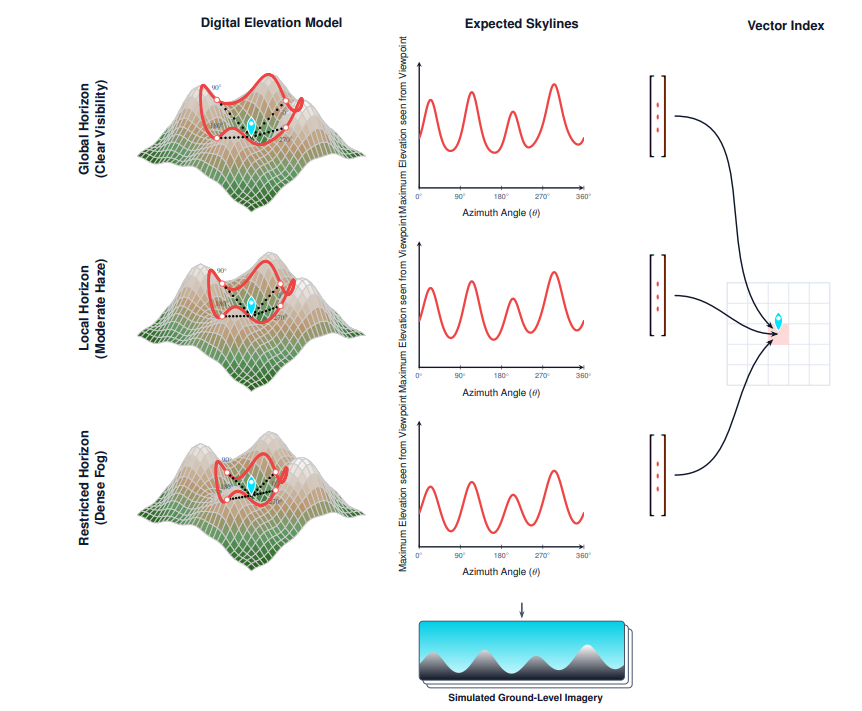
\includegraphics[width=0.85\textwidth]{src/images/page1.png} 
        \par \vspace{0.5em}
        \small \textbf{System Block Diagram:} Overview of the database generation and matching pipeline.
    \end{center}
\end{frame}

\begin{frame}{Methodology - [2] (Working Principle)}
    \begin{itemize}
        \item \textbf{Geometric Uniqueness:} Mountain skylines are permanent and unique landmarks that encode the observer's position.
        \item \textbf{Database-Query Matching:} The system matches the skyline extracted from a photo against a pre-computed database of synthetic horizons.
        \item \textbf{Offline Execution:} Coordinates are resolved by local search within the device without needing GPS or cellular data.
        \item \textbf{Absolute Elevation Signal:} Uses raw elevation values which carry strong discriminative signals for accurate positioning.
    \end{itemize}
\end{frame}

\begin{frame}{Methodology - [3] (Operational Workflow)}
    \begin{itemize}
        \item \textbf{Step 1 (Pre-processing):} Synthesis of 360-degree horizon profiles from DEM using ray-casting.
        \item \textbf{Step 2 (Segmentation):} Detecting sky-terrain boundary using a U-Net model.
        \item \textbf{Step 3 (Matching):} Fast global search using FFT-based Euclidean distance.
        \item \textbf{Step 4 (Refinement):} Fine-tuning the best candidates using Dynamic Time Warping (DTW).
        \item \textbf{Step 5 (Output):} Returning predicted Lat/Long and camera heading.
    \end{itemize}
\end{frame}

\begin{frame}{Methodology - [4] (Flow Of Proposed System)}
    \begin{center}
        \vspace{0.5em}
        % Changed from .tex to .png
        % Used height constraint here because flowcharts are often tall
        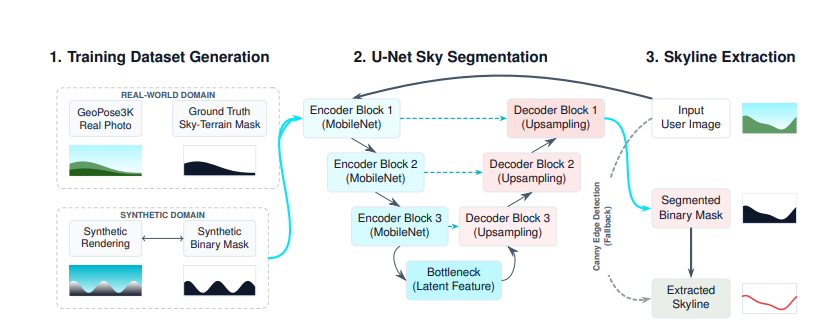
\includegraphics[height=0.7\textheight]{src/images/page2.png} 
        \par \vspace{0.5em}
        \small \textbf{Flowchart:} Pipeline from raw photo input to extracted skyline mask.
    \end{center}
\end{frame}

\begin{frame}{Methodology - [5] (Hardware Requirement)}
    \begin{itemize}
        \item \textbf{Training Host:} Workstation with CUDA-enabled GPU for training the segmentation model.
        \item \textbf{Deployment Target:} Mid-range Android smartphone for offline search.
        \item \textbf{Storage:} ~80 MB RAM/Disk space for storing 4,800 horizon viewpoints.
        \item \textbf{Camera:} Standard smartphone camera for image acquisition.
    \end{itemize}
\end{frame}

\begin{frame}{Methodology - [6] (Software Requirement)}
    \begin{itemize}
        \item \textbf{Programming Language:} Python (Development), C++ (Android Deployment).
        \item \textbf{ML Libraries:} PyTorch (Model training), NumPy/SciPy (Signal processing).
        \item \textbf{Computer Vision:} OpenCV for image manipulation and edge detection.
        \item \textbf{Libraries:} HORAYZON (Ray-casting), Android NDK (Deployment).
    \end{itemize}
\end{frame}

\begin{frame}{Methodology - [7] (Machine Learning Architecture)}
    \begin{itemize}
        \item \textbf{Model:} U-Net architecture for robust binary segmentation.
        \item \textbf{Encoder:} MobileNet-V3 backbone for lightweight and fast processing.
        \item \textbf{Objective:} To segment query photographs into sky and terrain masks even under poor lighting.
        \item \textbf{Fallback:} Canny Edge detection for low-confidence outputs.
    \end{itemize}
\end{frame}

\begin{frame}{Methodology - [8] (Algorithm Architecture)}
    \begin{center}
        \vspace{1em}
        % Changed from .tex to .png
        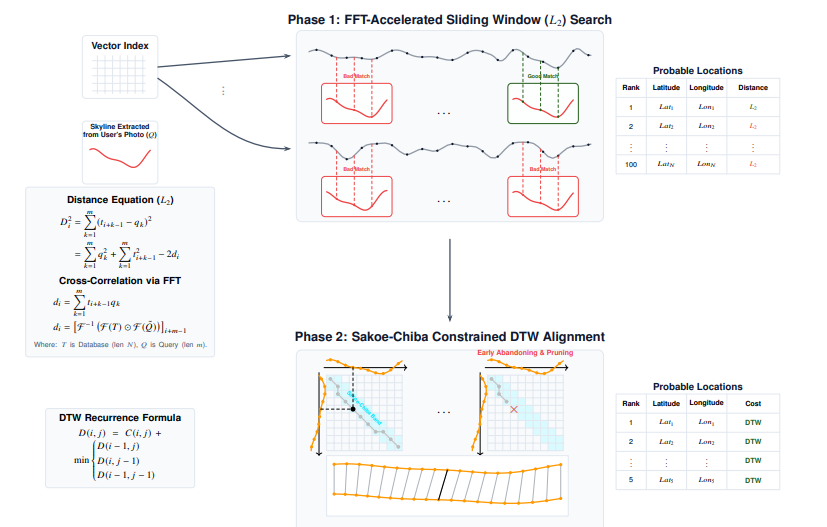
\includegraphics[width=0.9\textwidth]{src/images/page3.png} 
        \par \vspace{0.5em}
        \small \textbf{Algorithm Architecture:} Two-stage engine showing FFT-Sliding Window and DTW refinement.
    \end{center}
\end{frame}

\begin{frame}{Methodology - [9] (Dataset Preparation)}
    \begin{itemize}
        \item \textbf{Real Data:} GeoPose3K (3,000 labeled alpine images) for pre-training.
        \item \textbf{Synthetic Data:} Khumbu renderings generated from Copernicus GLO-30 DEM.
        \item \textbf{Ground Truth:} 45,000+ geotagged panoramas from Google Street View's Everest Trail.
        \item \textbf{Augmentation:} Procedural fog textures to simulate Himalayan weather.
    \end{itemize}
\end{frame}

\begin{frame}{Methodology - [10] (Snapshot of Dataset)}
    \begin{center}
        \vspace{1em}
        % You can also use an image here if you have one (e.g. dataset_sample.png)
        \fbox{\parbox{0.8\textwidth}{\centering
                \vspace{1cm}
                \textbf{GeoPose3K \& Khumbu Synthetic Images}\\
                \vspace{0.5em}
                (Input Image $\rightarrow$ Binary Mask $\rightarrow$ Skyline Vector)
                \vspace{1cm}
            }}
        \par \small \textbf{Snapshot:} Examples of the sky-terrain segmentation training data.
    \end{center}
\end{frame}

\begin{frame}{Methodology - [11] (Model Training)}
    \begin{itemize}
        \item \textbf{Strategy:} Pre-training on alpine data and fine-tuning on synthetic Khumbu terrain.
        \item \textbf{Optimization:} Adam optimizer with Cross-Entropy loss for pixel-level classification.
        \item \textbf{Evaluation:} Accuracy measured by grid-cell assignment on the test set.
        \item \textbf{Generalization:} Train/test splits made at the panorama level to avoid data leakage.
    \end{itemize}
\end{frame}